\documentclass{beamer}
\mode<presentation> {
%\usetheme{default}
%\usetheme{AnnArbor}
%\usetheme{Antibes}
%\usetheme{Bergen}
%\usetheme{Berkeley}
%\usetheme{Berlin}
%\usetheme{Boadilla}
%\usetheme{CambridgeUS}
%\usetheme{Copenhagen}
%\usetheme{Darmstadt}
%\usetheme{Dresden}
%\usetheme{Frankfurt}
%\usetheme{Goettingen}
%\usetheme{Hannover}
%\usetheme{Ilmenau}
%\usetheme{JuanLesPins}
%\usetheme{Luebeck}
%\usetheme{Madrid}
%\usetheme{Malmoe}
%\usetheme{Marburg}
%\usetheme{Montpellier}
%\usetheme{PaloAlto}
\usetheme{Pittsburgh}
%\usetheme{Rochester}
%\usetheme{Singapore}
%\usetheme{Szeged}
%\usetheme{Warsaw}

%\usecolortheme{albatross}
%\usecolortheme{beaver}
%\usecolortheme{beetle}
%\usecolortheme{crane}
%\usecolortheme{dolphin}
%\usecolortheme{dove}
%\usecolortheme{fly}
%\usecolortheme{lily}
%\usecolortheme{orchid}
%\usecolortheme{rose}
%\usecolortheme{seagull}
%\usecolortheme{seahorse}
%\usecolortheme{whale}
%\usecolortheme{wolverine}

%\setbeamertemplate{footline} % To remove the footer line in all slides uncomment this line
\setbeamertemplate{footline}[page number] % To replace the footer line in all slides with a simple slide count uncomment this line
\setbeamertemplate{navigation symbols}{} % To remove the navigation symbols from the bottom of all slides uncomment this line
}

\usepackage{graphicx} % Allows including images
\usepackage{booktabs} % Allows the use of \toprule, \midrule and \bottomrule in tables
\usepackage{cancel}

\usepackage{amsmath}
%\usepackage{amsthm}
\usepackage{amssymb}

\usepackage{accents}
%\usepackage{thmtools}
\usepackage{mathtools}
\usepackage{graphicx}
\usepackage{tikz}
\usepackage{pgfplots}
\usepackage{natbib}



\DeclareMathOperator*{\argmin}{\arg\!\min}
\DeclareMathOperator*{\argmax}{\arg\!\max}
\DeclareMathOperator{\E}{\mathbb{E}}
\DeclareMathOperator{\p}{\mathbb{P}}
\DeclareMathOperator{\pr}{\mathbb{P}}
\newlength{\dhatheight}
\newcommand{\doublehat}[1]{%
    \settoheight{\dhatheight}{\ensuremath{\hat{#1}}}%
    \addtolength{\dhatheight}{-0.15ex}%
    \hat{\vphantom{\rule{1pt}{\dhatheight}}%
    \smash{\hat{#1}}}}

%----------------------------------------------------------------------------------------
%	TITLE PAGE
%----------------------------------------------------------------------------------------

\title[An Engineered Empirical Bernstein Bound]{An Engineered Empirical Bernstein Bound} % The short title appears at the bottom of every slide, the full title is only on the title page

\author[shortname]{Mark Alexander Burgess\inst{1} \and Archie C. Chapman\inst{2} \and Paul Scott\inst{1}}
\institute[institutions_short]{\inst{1} Australian National University\\ College of Engineering and Computer Science \and %
                      \inst{2} University of Queensland\\ School of Information Technology and Electrical Engineering \\	
\medskip
\textit{mark.burgess@anu.edu.au, markburgess1989@gmail.com} \\
\textit{archie.chapman@uq.edu.au}\\
\textit{paul.scott@anu.edu.au}
}


\date{\today} % Date, can be changed to a custom date

\begin{document}

\begin{frame}
\titlepage % Print the title page as the first slide
\end{frame}

%\begin{frame}
%\frametitle{Overview} % Table of contents slide, comment this block out to remove it
%\tableofcontents % Throughout your presentation, if you choose to use \section{} and \subsection{} commands, these will automatically be printed on this slide as an overview of your presentation
%\end{frame}

%----------------------------------------------------------------------------------------
%	PRESENTATION SLIDES
%----------------------------------------------------------------------------------------

%------------------------------------------------
\section{What are Empirical Bernstein Bounds} % Sections can be created in order to organize your presentation into discrete blocks, all sections and subsections are automatically printed in the table of contents as an overview of the talk
%------------------------------------------------

\subsection{dumb example via Chebyshev's Inequality} % A subsection can be created just before a set of slides with a common theme to further break down your presentation into chunks

\begin{frame}
\frametitle{What is an EBB}
An Empirical Bernstein Bound (EBB) is a bound on the error of your sampled statistics parameterised by their sample variances.\\
Why do we care?\\
\-\hspace{1cm}\\
\-\hspace{1cm} Because we are data scientists.\\
\-\hspace{1cm} We use sample statistics to compare information sets.
\end{frame}

\begin{frame}
\frametitle{Cooking An example EBB}
Lets walk through the process of creating a example (single-dimensional) EBB.\\
\begin{theorem}[Chebyshev's inequality]
for any random variable $X$ of mean $\mu$, with variance $\sigma^2$, then the error of $X$ about $\mu$ is probability bounded:
$$ \p\left(|X-\mu|\ge k\sigma\right)\le\frac{1}{k^2} $$
\end{theorem}
Assumes $X$ ...\textit{has a variance}...!
\end{frame}

\begin{frame}
\frametitle{Cooking An example EBB}
Using $\text{Var}(aX+bY)=a^2\text{Var}(X)+b^2\text{Var}(Y)$:
\begin{theorem}[Chebyshev's inequality for samples]
for any sample mean $\hat{\mu}$ of random variable $X$ of mean $\mu$, with variance $\sigma^2$, then the error is bounded:
$$ \p\left(|\hat{\mu}-\mu|\ge k\right)\le\frac{\sigma^2}{nk^2} $$
\end{theorem}
So simple. So usefull.\\
\-\hspace{1cm} ...If only we knew $\sigma^2$
\end{frame}


\begin{frame}
\frametitle{Cooking an example EBB}
But what we do have the sample variance\\ $\hat{\sigma}^2 = \frac{1}{n-1}\sum(x_i-\hat{\mu})^2$\\
so... perhaps...
$$ \p\left(|\hat{\mu}-\mu|\ge k\right)\lessapprox\frac{\hat{\sigma}^2}{nk^2} $$
Nobody will shoot you.\\
If you only have minimal assumptions, then...
$$ \p\left(|\hat{\mu}-\mu|\ge k\right)\le ~??? (n,k,\hat{\sigma}^2) $$
...thinking time...\\
That is an Empirical Bernstein Bound.
\end{frame}


\begin{frame}
\frametitle{Cooking an example EBB}
Well... we have to articulate the error on the variance.\\
Lets recycle Chebyshev's inequality again:
$$ \p\left(|\hat{\sigma}^2-\sigma^2|\ge t\sqrt{\text{Var}(\hat{\sigma}^2)}\right)\le\frac{1}{t^2} $$
And doing some algebra:
$$ \text{Var}(\hat{\sigma}^2) = \frac{3-n}{n(n-1)}\sigma^2 + \frac{1}{n}\mu_4$$
where $\mu_4$ is the forth central moment $\E[(X-\mu)^4]$.\\
\end{frame}


\begin{frame}
\frametitle{Cooking an example EBB}
For $n\ge 3$ the first term is non-positive, so lets get rid of it.
$$ \text{Var}(\hat{\sigma}^2) \le \cancel{\frac{3-n}{n(n-1)}\sigma^2} + \frac{1}{n}\mu_4$$
So therefore:
$$ \p\left(|\hat{\sigma}^2-\sigma^2|\ge t\sqrt{\frac{1}{n}\mu_4}\right)\le\frac{1}{t^2} $$
A double sided inequality works one sided too, so:
$$ \p\left(\sigma^2\ge \hat{\sigma}^2 + t\sqrt{\frac{1}{n}\mu_4}\right)\le\frac{1}{t^2} $$
This is a horrible horrible bound on the variance - just so you know.
\end{frame}

\begin{frame}
\frametitle{Cooking an example EBB}
We have our horrible tokien bound for the variance:
$$ \p\left(\sigma^2\ge \hat{\sigma}^2 + t\sqrt{\frac{1}{n}\mu_4}\right)\le\frac{1}{t^2} $$
And our sample chernoff bound using the variance:
$$ \p\left(|\hat{\mu}-\mu|\ge k\right)\le\frac{\sigma^2}{nk^2} $$
How do we combine the two?

\end{frame}

\begin{frame}
\frametitle{Cooking an example EBB}
\begin{lemma}[Probability Union]\label{prob_union}
For any random variables $a,b$ and $c$:
\[\p(a>c) \; \le \; \p(a>b) + \p(b>c)\]
\end{lemma}
\-\hspace{1cm}\\
\-\hspace{1cm}\\
\-\hspace{1cm}\\
Ok.. which gives us:
$$ \p\left(|\mu-\hat{\mu}|\ge \frac{k}{\sqrt{n}}\sqrt{\hat{\sigma}^2 + t\sqrt{\frac{\mu_4}{n}}}\right)\le\frac{1}{k^2}+\frac{1}{t^2} $$
\end{frame}

\begin{frame}
\frametitle{Cooking an example EBB}
Which we can polish up by setting $k=t$ (because why not)
and scaling gives:
$$ \p\left(|\mu-\hat{\mu}|\ge \sqrt{\frac{2}{nk}}\sqrt{\hat{\sigma}^2 + \sqrt{\frac{2\mu_4}{nk}}}\right)\le k $$

And this completes the derivation of an example of an Empirical Bernstein Bound. (HORRIBLE!)\\
\-\hspace{1cm}\\


And if we have some dummy upper bound for $\mu_4$ we are done.\\
eg. if the data is bounded with a width $D$ then $\mu_4\le D^4/16$
\end{frame}



\begin{frame}
\frametitle{Ok - so why do we care?}
Concentration inequalities are applied in a range of contexts for prediction, machine learning and hypothesis testing tasks, including:\\

\begin{itemize}
\item change detection - \cite{KiferShaiGehrke2004,8000571}
\item classification in data streams - \cite{Zia-UrRehman2012}
\item outlier analysis in large databases - \cite{Aggarwal2015}
\item online optimisation - \cite{FlaxmanKalaiMcMahan2005,AgarwalDekelXiao2010}; 
\item online prediction and learning problems - \cite{Cesa-BianchiLugosi2006,%Maron1997,
Mnih:2008:EBS:1390156.1390241,DBLP:conf/aaai/ThomasTG15,Maurer50empiricalbernstein},
\item in settings with bandit feedback - \cite{AuerCesa-BianchiEtal_SIAM2003,AudibertBubeck_COLT2009,Tran-ThanhChapmanRJ_AAAI2009}.
\end{itemize}
Even by atendees at this conference...
\end{frame}



\subsection{Other concentration inequalities}

\begin{frame}
\frametitle{Ok - so why do we care?}
In various applications, Hoeffding's inequality is often used:
\begin{theorem}[Hoeffding's inequality]\label{hoeffdings_inequality}
For $X$ is random variable with mean $\mu$, that is bounded $a\le X\le b$. Then for $D=b-a$ and any $t>0$, the sample mean $\hat{\mu}$ of $n$ independent samples of $X$ is probability bounded:
$$\p(\hat{\mu}-\mu\ge t)\le \exp\left(\frac{-2nt^2}{D^2}\right)$$
$$\text{ie.}\quad\quad\p\left(\hat{\mu}-\mu\ge \sqrt{\frac{D\log(1/t)}{2n}}\right)\le t$$
\end{theorem}
And hoeffding's inequality is not sensitive to the sample variance.
\end{frame}

\begin{frame}
\frametitle{Ok - so why do we care?}
And existing published EBBs are modified Hoeffding's inequality:
\begin{theorem}[\cite{Maurer50empiricalbernstein}]\label{MandPsEBB}
Let $X$ be bounded within a width $D$.  Then the sample mean $\hat{\mu}$ and sample variance $\hat{\sigma}^2$ of $n$ samples, are probability bounded:
$$ \p\left(\mu-\hat{\mu}\ge\sqrt{\frac{2\hat{\sigma}^2\log(2/t)}{n}}+\frac{7D\log(2/t)}{3(n-1)}\right)\le t $$
\end{theorem}

\begin{theorem}[\cite{10.1007/978-3-540-75225-7_15}]
In exactly the same context as in Theorem \ref{MandPsEBB}
$$ \p\left(\mu-\hat{\mu}\ge\sqrt{\frac{2\hat{\sigma}^2\log(3/t)}{2n}} + \frac{3D\log(3/t)}{2n}\right) \le t $$
\end{theorem}
\end{frame}



\section{How to improve}

\begin{frame}
\frametitle{To start with stronger bounds}
For a start are stronger versions of Hoeffding's inequality, particularly in all the various literature on Hypergeometric tail inequalities.
%\begin{theorem}[Hypergeometric bounds, Also derived from Hoeffding's inequality]\label{hoeffdings_inequality22}
%Let $X$ be a real-valued random variable that is bounded $a\le X\le b$, with a mean $\mu$ of zero.  Then for $t>0$, the mean $\hat{\mu}$ of $n$ independent samples of $X$ is probability bounded by:
%$$ \p(\hat{\mu}-\mu\ge t)\le \left( \frac{b}{D}\left(\frac{b(a-t)}{a(b-t)}\right)^{\frac{a-t}{D}} -\frac{a}{D}\left(\frac{b(a-t)}{a(b-t)}\right)^{\frac{b-t}{D}}  \right)^n $$
%\end{theorem}

\begin{theorem}[Also credited to Hoeffding]
Let $X$ be a real-valued random variable that is bounded $0\le X\le 1$, with mean $\mu$. Then for $t>0$, the mean $\hat{\mu}$ of $n$ independent samples of $X$ is probability bounded by:
\begin{equation*}\p(\hat{\mu}-\mu\ge t)\le \left[\left(\frac{1-\mu}{1-t-\mu}\right)^{1-t-\mu}  \left(\frac{\mu}{t+\mu}\right)^{t+\mu}\right]^n
\end{equation*}
\end{theorem}

But if you add variance information then you can potentially get even stronger results.
\end{frame}


\begin{frame}
\frametitle{To improve you choose stronger bounds}
Obviously there is Chebyschev's inequality,\\
And there is the various Bernstein inequalities.\\
But we can do better.

\begin{theorem}[Bennett's inequality]\label{hoeffdings1}
Let $X$ be a real-valued random variable with a mean of zero and variance $\sigma^2$, that is bounded $a\le X\le b$. 
Then for $t>0$, the mean $\hat{\mu}$ of $n$ samples of $X$ is probability bounded by:
\begin{equation*}\label{eq_no2}\p(\hat{\mu}\ge t)\le 
\left(\left(\frac{\frac{\sigma^2}{b^2}}{\frac{\sigma^2}{b^2}+\frac{t}{b}}\right)^{\frac{\sigma^2}{b^2}+\frac{t}{b}}
\left(\frac{1}{1-\frac{t}{b}}\right)^{1-\frac{t}{b}}\right)^{\frac{n}{\frac{\sigma^2}{b^2}+1}}
\end{equation*}
\end{theorem}
\end{frame}


\begin{frame}
\frametitle{Research Question?}
What if we started with a good concentration inequality \\(ie. Bennett's), and then incorporated strong sample variance information?\\
\-\hspace{1cm}\\
If we engineered this, what kind of improvement would it offer?
\end{frame}



\begin{frame}
Just like with our Chebyschev's inequality bound, we need a good bound on the variance - not easy to make.\\
\-\hspace{1cm}\\
%We decomose the variance into mean squared and sample squares:

\begin{lemma}[Variance Decomposition]\label{variance1}
For $n$ samples, the sample mean $\hat{\mu}$, sample variance $\hat{\sigma}^2$, and average of sample squares $\hat{\sigma}_0^2$, the following relationship holds:
$$ \hat{\sigma}_0^2=\hat{\mu}^2+\frac{n-1}{n}\hat{\sigma}^2 $$
\end{lemma}
\-\hspace{1cm}\\
We cant easily develop a strong bound for $\hat{\sigma}^2$\\ But we can develop good bounds for $\hat{\mu}^2$ and also $\hat{\sigma}_0^2$.
\end{frame}

\begin{frame}
%So we develop a good bound for the sample squares:
\begin{lemma}[Sample square bound]\label{sample_squares}
Let $X$ be a real-valued random variable with a mean of zero and variance $\sigma^2$, that is bounded $a\le X\le b$, if $d=\max(b,-a)$ then for $y>0$, the mean of sample squares $\hat{\sigma}_0^2=\frac{1}{n}\sum_ix_i^2$ is probability bounded:
\begin{equation*}\p(\sigma^2 - \hat{\sigma}_0^2> y) \le \left(
\left(\frac{1-\frac{\sigma^2}{d^2}}{1+\frac{y}{d^2}-\frac{\sigma^2}{d^2}}\right)^{1+\frac{y}{d^2}-\frac{\sigma^2}{d^2}}
\left(\frac{\frac{\sigma^2}{d^2}}{\frac{\sigma^2}{d^2}-\frac{y}{d^2}}\right)^{\frac{\sigma^2}{d^2}-\frac{y}{d^2}}
\right)^n
\end{equation*}
\end{lemma}
\-\hspace{1cm}\\
Now these kind of equations are impossible to manipulate.\\
Which is the cost of not using simplifying approximations.
\end{frame}


\begin{frame}
Since the variance is a more general \textit{function} of random variables, There are primarily two other processes to bound similar functions.
\begin{enumerate}
\item Efron-Stein method to bound the variance, with choice of a bound like Chebyshev's inequality.
\item Entropy methods via the Herbst argument - quasi information theoretic.
\end{enumerate}
the first yields similar inequality to what we just previously derived:
$$ \text{Var}(\hat{\sigma}^2) \le \frac{5-n}{n(n-1)}\sigma^2 + \frac{1}{n}\mu_4 $$
The second has been developed by others, \cite{MR2245497}:
$$ \p(\sigma^2 - \hat{\sigma}^2>w) \le \exp\left(\frac{-(n-1)w^2}{2\sigma^2D^2}\right) $$
For our engineering task, nothing prohibits taking the best\\(ie. minima) of several different bounds. 
\end{frame}


\begin{frame}
TL:DR the algebra is the same as our Chebyshev's bound.\\ But using numerics to do intractable algebra.\\
The ingredients:
\begin{itemize}
\item Variance Decomposition:
$ \hat{\sigma}_0^2=\hat{\mu}^2+\frac{n-1}{n}\hat{\sigma}^2 $
\item Probability Union:
$\p(a>c) \; \le \; \p(a>b) + \p(b>c)$
\item Bennett's inequality:
\begin{equation*}\label{eq_no2}\p(\hat{\mu}\ge t)\le 
\left(\left(\frac{\frac{\sigma^2}{b^2}}{\frac{\sigma^2}{b^2}+\frac{t}{b}}\right)^{\frac{\sigma^2}{b^2}+\frac{t}{b}}
\left(\frac{1}{1-\frac{t}{b}}\right)^{1-\frac{t}{b}}\right)^{\frac{n}{\frac{\sigma^2}{b^2}+1}}
\end{equation*}
\item Our own sample-squares inequality:
\begin{equation*}\p(\sigma^2 - \hat{\sigma}_0^2> y) \le \left(
\left(\frac{1-\frac{\sigma^2}{d^2}}{1+\frac{y}{d^2}-\frac{\sigma^2}{d^2}}\right)^{1+\frac{y}{d^2}-\frac{\sigma^2}{d^2}}
\left(\frac{\frac{\sigma^2}{d^2}}{\frac{\sigma^2}{d^2}-\frac{y}{d^2}}\right)^{\frac{\sigma^2}{d^2}-\frac{y}{d^2}}
\right)^n
\end{equation*}
\end{itemize}
\end{frame}

\begin{frame}

Do all the numerics and then \textit{at the end} safely fit a simple envelope over the results to get a take-away equation.\\
\-\hspace{1cm}\\ An example equation we ended up with was:
 
\begin{equation*}\label{eq:prob_bound} \p\left(\mu-\hat{\mu}\ge \frac{D}{\sqrt{n}}\; 
\footnotesize
\left(\begin{matrix*}[c]
\frac{3}{5}\sqrt{\min\left[1,\frac{\hat{\sigma}^2}{D^2}+\frac{25}{n}\right]} \\+ \ln\left(\max\left[1,n\left(1-\frac{\hat{\sigma}^2}{D^2}\right)\right]\right)^{-4}\end{matrix*}
\normalsize
\right)\right) 
\le 0.5 \end{equation*}
\end{frame}

\section{Some Results}

\subsection{Bandits and UCB method}

\begin{frame}
\frametitle{Does it work? - Bandits}

Concentration inequalities are used to generate upper confidence bounds in the \textit{upper-confidence bound} (UCB) method bandit problems.

At each time-step, a player has to choose which of the arms to pull to get the most reward.
Under UCB, the arm with the greatest upper confidence bound on the estimated mean of its reward is selected.

Specifically, the general form of UCB methods is to define a \textit{confidence interval}, $CI$ on the estimate of the mean:
\[
\mathbb{P}\left(\mu - \hat{\mu} \ge CI \right) \le y
\]
where $y$ is a confidence level.
\end{frame}



\begin{frame}
\frametitle{Some Bandits Results}


\begin{figure}
    \centering
	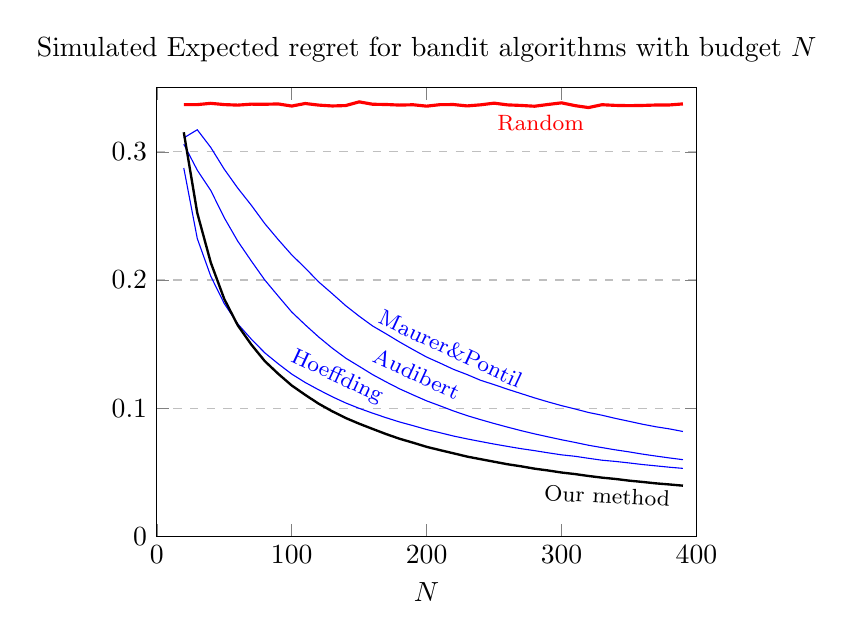
\begin{tikzpicture}
	\begin{axis}[
		title={Simulated Expected regret for bandit algorithms with budget $N$},
		xlabel={$N$},
		xmin=0, xmax=400,
		ymin=0, ymax=0.35,
		ymajorgrids=true,
		grid style=dashed
	]
	\addplot[blue] coordinates {
(20, 0.310951130364) (30, 0.317304721799) (40, 0.303506740539) (50, 0.286502047961) (60, 0.271750798627) (70, 0.258441105474) (80, 0.244084337607) (90, 0.23154222192) (100, 0.21962674765) (110, 0.209364293145) (120, 0.19849795256) (130, 0.189366124494) (140, 0.179985057504) (150, 0.17175192486) (160, 0.164084467112) (170, 0.15795328799) (180, 0.151595586119) (190, 0.145627208562) (200, 0.139841473843) (210, 0.135131674343) (220, 0.130210872033) (230, 0.126186563148) (240, 0.121707370459) (250, 0.118323364967) (260, 0.114727672756) (270, 0.11135242178) (280, 0.107973086348) (290, 0.104854372357) (300, 0.101926121277) (310, 0.0993107935735) (320, 0.0965791677494) (330, 0.0944273468526) (340, 0.0919468150041) (350, 0.0897017110445) (360, 0.0874165452919) (370, 0.085411858643) (380, 0.0837605537036) (390, 0.0817399520606)
		}node[pos=0.52](endofplotsquare){} ;
		\node [blue,above,rotate=-25] at (endofplotsquare) {\footnotesize Maurer\&Pontil};
	\addplot[red,line width=0.4mm] coordinates {
(20, 0.336942958587) (30, 0.336937645823) (40, 0.33793528862) (50, 0.336950104881) (60, 0.336542611243) (70, 0.337280819312) (80, 0.337200777509) (90, 0.337451863926) (100, 0.335809963856) (110, 0.337793875156) (120, 0.33654914298) (130, 0.335875820615) (140, 0.336188909491) (150, 0.339081235627) (160, 0.337206338081) (170, 0.337020887335) (180, 0.336563951732) (190, 0.336823591936) (200, 0.335728527085) (210, 0.336906574325) (220, 0.336981316156) (230, 0.33591692432) (240, 0.336764452534) (250, 0.338074323749) (260, 0.336715624161) (270, 0.336287747782) (280, 0.335670715253) (290, 0.337037990821) (300, 0.338315025894) (310, 0.336139218506) (320, 0.334622390817) (330, 0.336859134941) (340, 0.336317904597) (350, 0.336124307504) (360, 0.336277839902) (370, 0.336613274) (380, 0.336662753516) (390, 0.337483689505)
		}node[pos=0.715](endofplotsquare){} ;
		\node [red,below] at (endofplotsquare) {\footnotesize Random};
	\addplot[blue] coordinates {
(20, 0.28743290587) (30, 0.232382220095) (40, 0.20296927431) (50, 0.181606720226) (60, 0.165745102011) (70, 0.153907558509) (80, 0.143186137085) (90, 0.134590089348) (100, 0.126573002174) (110, 0.119992831407) (120, 0.11427869441) (130, 0.108890725408) (140, 0.104018433267) (150, 0.0998081258891) (160, 0.0960210094774) (170, 0.0924770288966) (180, 0.0891490256632) (190, 0.0862832212207) (200, 0.0832737235473) (210, 0.0807582587196) (220, 0.0781651915387) (230, 0.0759558632013) (240, 0.0739131187913) (250, 0.0719286269452) (260, 0.0700910030206) (270, 0.0683275770601) (280, 0.0667819025719) (290, 0.0650880008227) (300, 0.063500206177) (310, 0.0623834758598) (320, 0.0608073686435) (330, 0.0593185615513) (340, 0.0583541183652) (350, 0.0571870323598) (360, 0.0559368431009) (370, 0.054899877847) (380, 0.0538413306667) (390, 0.052941312716)
		}node[pos=0.29](endofplotsquare){} ;
		\node [blue,above,rotate=-25] at (endofplotsquare) {\footnotesize Hoeffding};
	\addplot[blue] coordinates {
(20, 0.306061843642) (30, 0.285754524727) (40, 0.269931278197) (50, 0.248615326378) (60, 0.230327866882) (70, 0.214922429349) (80, 0.200054374281) (90, 0.187439612189) (100, 0.175026770923) (110, 0.165017888537) (120, 0.155510023043) (130, 0.146850970099) (140, 0.139027366099) (150, 0.132617934825) (160, 0.126130658589) (170, 0.120431591885) (180, 0.115019877981) (190, 0.110269427886) (200, 0.105649535257) (210, 0.101741763249) (220, 0.0977283222415) (230, 0.0941251046786) (240, 0.0909714233319) (250, 0.0879807411491) (260, 0.0851390725522) (270, 0.0824012109451) (280, 0.079883684561) (290, 0.0775606819917) (300, 0.0752888280648) (310, 0.0732028631441) (320, 0.070993850246) (330, 0.069161594945) (340, 0.0673921094242) (350, 0.06583053422) (360, 0.0640749729154) (370, 0.0625422168091) (380, 0.0610836359114) (390, 0.0597357326982)
		}node[pos=0.35](endofplotsquare){} ;
		\node [blue,above right, rotate=-25] at (endofplotsquare) {\footnotesize Audibert};
	\addplot[line width=0.30mm] coordinates {
(20, 0.315351878837) (30, 0.252310598394) (40, 0.21365051234) (50, 0.185173245204) (60, 0.164633657836) (70, 0.149662482149) (80, 0.136725328307) (90, 0.126768907712) (100, 0.117664528623) (110, 0.110326598166) (120, 0.103415978409) (130, 0.0975188110085) (140, 0.0922740034531) (150, 0.0878113744221) (160, 0.0837255031) (170, 0.0797008178449) (180, 0.0760441489445) (190, 0.0729725631572) (200, 0.0697582108496) (210, 0.0671583991446) (220, 0.06468719194) (230, 0.0621409299865) (240, 0.0601285592881) (250, 0.0581341532097) (260, 0.0561603237441) (270, 0.0545519043883) (280, 0.0527161522742) (290, 0.0513002710141) (300, 0.0497036485461) (310, 0.0484855329667) (320, 0.0470042219926) (330, 0.045703669572) (340, 0.0446693501732) (350, 0.0433740760739) (360, 0.0423482852895) (370, 0.0412370883341) (380, 0.0403742986427) (390, 0.0394378538536)
		}node[pos=0.85](endofplotsquare){} ;
		\node [below,rotate=-3] at (endofplotsquare) {\footnotesize Our method};
	\end{axis}
	\end{tikzpicture}
	\vspace{-5pt}
	\caption{The expected regret of bandit algorithms and a baseline method in the example bandit problem: UCB method using our bound \eqref{eq:prob_bound}, Hoeffding's, Audibert et.al's, and Maurer \& Pontil's inequalities; and method of uniform randomly choosing an arm.}
	\label{biggraph44}
\end{figure}


\end{frame}





\subsection{In comparrison with perfect variance information}

\begin{frame}
\frametitle{In comparrison with other EBBs?}
\begin{figure}[]{}
    \centering
	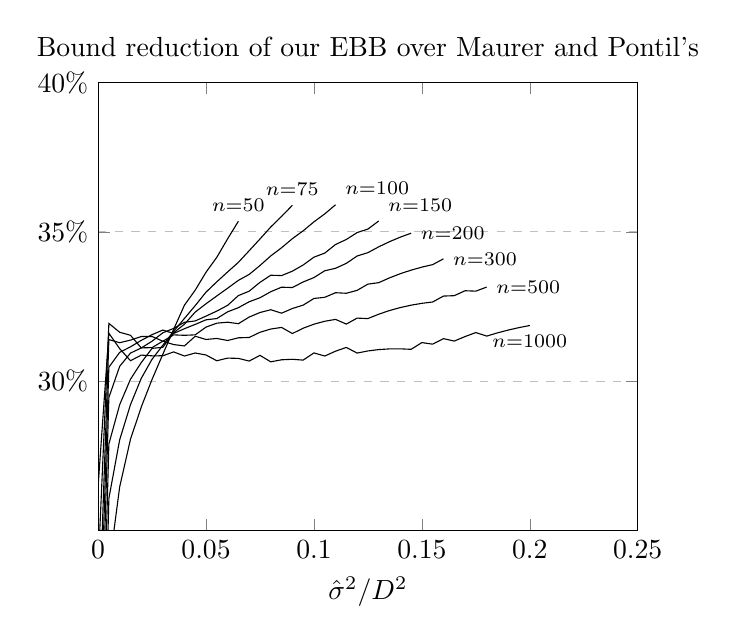
\begin{tikzpicture}
	\begin{axis}[
		title={Bound reduction of our EBB over  Maurer and Pontil’s},
		xlabel={$\hat{\sigma}^2/D^2$},
		xmin=0, xmax=0.25,
		ymin=25, ymax=40,
		xtick={0,0.05,0.1,0.15,0.2,0.25},
		ytick={30,35,40},
		yticklabel=$\pgfmathprintnumber{\tick}\%$,
		ymajorgrids=true,
		grid style=dashed,
		xticklabel style={/pgf/number format/fixed},
	]
	\addplot[] coordinates {
(0.0, 10.038489469957923)(0.005, 23.729228874038338)(0.01, 26.46795119155083)(0.015, 28.061119743643296)(0.02, 29.141938583623652)(0.025, 30.066155991693723)(0.03, 30.907282335052788)(0.035, 31.738722848538305)(0.04, 32.54914392836502)(0.045, 33.05291848928947)(0.05, 33.651509619741496)(0.055, 34.151805087746446)(0.06, 34.768247610158575)(0.065, 35.35764746719292)
		}node[pos=1.0](endofplotsquare){} ;
	\node [above] at (endofplotsquare) {$\scriptstyle n=50$};
	\addplot[] coordinates {
(0.0, 12.591458904845746)(0.005, 26.08582516018055)(0.01, 28.044488963240152)(0.015, 29.219014176778845)(0.02, 30.101019545112305)(0.025, 30.739739304373572)(0.03, 31.209391146592484)(0.035, 31.67459564986504)(0.04, 32.10560417423678)(0.045, 32.53522214247566)(0.05, 32.98480753922602)(0.055, 33.33123349968554)(0.06, 33.66064263107598)(0.065, 33.983296057116895)(0.07, 34.371432119724126)(0.075, 34.76400092304011)(0.08, 35.165771922230526)(0.085, 35.51929445366766)(0.09, 35.890640326573575)
		}node[pos=1.0](endofplotsquare){} ;
	\node [above] at (endofplotsquare) {$\scriptstyle n=75$};
	\addplot[] coordinates {
(0.0, 14.817995440815901)(0.005, 27.90751007185735)(0.01, 29.219819451516923)(0.015, 30.070639062533996)(0.02, 30.629290720122317)(0.025, 31.104197838170627)(0.03, 31.14038996461402)(0.035, 31.62526607199946)(0.04, 31.911575841232846)(0.045, 32.3187069670152)(0.05, 32.59698646227685)(0.055, 32.85814963311234)(0.06, 33.115830685662)(0.065, 33.379908028841236)(0.07, 33.578110917203176)(0.075, 33.87653264786374)(0.08, 34.19803078792182)(0.085, 34.470564003329045)(0.09, 34.774201537103245)(0.095, 35.03784322660741)(0.1, 35.337583634279)(0.105, 35.60362789769355)(0.11, 35.90890662248758)
		}node[pos=1.0](endofplotsquare){} ;
	\node [above right] at (endofplotsquare) {$\scriptstyle n=100$};
	\addplot[] coordinates {
(0.0, 17.342661445161745)(0.005, 29.461247776997926)(0.01, 30.502124709956824)(0.015, 30.94634600450878)(0.02, 31.116833768989828)(0.025, 31.344627574353588)(0.03, 31.62499327739429)(0.035, 31.772139980592)(0.04, 31.975727165299386)(0.045, 32.02196228998142)(0.05, 32.183034431467235)(0.055, 32.352369659168474)(0.06, 32.54250416890406)(0.065, 32.87047963677422)(0.07, 33.017679271803296)(0.075, 33.31333732160584)(0.08, 33.55087101615144)(0.085, 33.53938459819124)(0.09, 33.68714872653657)(0.095, 33.89275583281304)(0.1, 34.15600891069251)(0.105, 34.290920495879966)(0.11, 34.57974857223946)(0.115, 34.747357884723435)(0.12, 34.97811379083637)(0.125, 35.09584827017029)(0.13, 35.36531839253051)
		}node[pos=1.0](endofplotsquare){} ;
	\node [above right] at (endofplotsquare) {$\scriptstyle n=150$};
	\addplot[] coordinates {
(0.0, 19.269181617386778)(0.005, 30.47328215171227)(0.01, 30.970505248952783)(0.015, 31.155076903228505)(0.02, 31.370737591330126)(0.025, 31.563153411429678)(0.03, 31.716924278688328)(0.035, 31.602163041853583)(0.04, 31.762160711176872)(0.045, 31.905759719654245)(0.05, 32.05956774531062)(0.055, 32.101874254626836)(0.06, 32.32639539364612)(0.065, 32.465858041087344)(0.07, 32.663895247621326)(0.075, 32.797586647322234)(0.08, 32.99998541625402)(0.085, 33.15092115439265)(0.09, 33.13907818080335)(0.095, 33.32527974281349)(0.1, 33.47347491095124)(0.105, 33.70030345616673)(0.11, 33.78337094262078)(0.115, 33.94866206353597)(0.12, 34.19406008169977)(0.125, 34.30666804274627)(0.13, 34.5014054670121)(0.135, 34.67351335871075)(0.14, 34.82497129829329)(0.145, 34.95753413863828)
		}node[pos=1.0](endofplotsquare){} ;
	\node [right] at (endofplotsquare) {$\scriptstyle n=200$};
	\addplot[] coordinates {
(0.0, 21.01455983414305)(0.005, 31.398323351742654)(0.01, 31.29316800287044)(0.015, 31.380044700971307)(0.02, 31.499573558604126)(0.025, 31.501955199548522)(0.03, 31.342388805161228)(0.035, 31.555898653589576)(0.04, 31.540720961712708)(0.045, 31.556719994430246)(0.05, 31.815518124296712)(0.055, 31.947447662218103)(0.06, 31.979020008525413)(0.065, 31.929950573976118)(0.07, 32.151946530365926)(0.075, 32.30372613153442)(0.08, 32.39631985663968)(0.085, 32.28147349936643)(0.09, 32.43775937546441)(0.095, 32.55064623256504)(0.1, 32.77372870056995)(0.105, 32.81284419609248)(0.11, 32.96572615770543)(0.115, 32.94748952790814)(0.12, 33.04474761150041)(0.125, 33.25359991684834)(0.13, 33.30204392434083)(0.135, 33.462830030160355)(0.14, 33.601886363972085)(0.145, 33.7211101175424)(0.15, 33.822185822075845)(0.155, 33.90661477833436)(0.16, 34.09961256888578)
		}node[pos=1.0](endofplotsquare){} ;
	\node [right] at (endofplotsquare) {$\scriptstyle n=300$};
	\addplot[] coordinates {
(0.0, 23.733576061543907)(0.005, 31.93999128292596)(0.01, 31.642400396531094)(0.015, 31.54212092349261)(0.02, 31.12052542652318)(0.025, 31.129819611252405)(0.03, 31.344098301521242)(0.035, 31.231838999520004)(0.04, 31.185453514912005)(0.045, 31.51029078782499)(0.05, 31.401697787018254)(0.055, 31.43592520457107)(0.06, 31.367624957687056)(0.065, 31.45753767654653)(0.07, 31.468778394474676)(0.075, 31.6423499409508)(0.08, 31.751037287923307)(0.085, 31.804794091938522)(0.09, 31.59991862434968)(0.095, 31.778311022724473)(0.1, 31.913384999263183)(0.105, 32.010501900631745)(0.11, 32.074189915872516)(0.115, 31.915973789453584)(0.12, 32.11613625130849)(0.125, 32.10053700848796)(0.13, 32.24708311545571)(0.135, 32.3692691037866)(0.14, 32.46936498795406)(0.145, 32.54937215145163)(0.15, 32.61106237732128)(0.155, 32.65601018366708)(0.16, 32.85390573088976)(0.165, 32.867317678660584)(0.17, 33.03199624865481)(0.175, 33.01872182909822)(0.18, 33.15487119563348)
		}node[pos=1.0](endofplotsquare){} ;
	\node [right] at (endofplotsquare) {$\scriptstyle n=500$};
	\addplot[] coordinates {
(0.0, 26.48466951022569)(0.005, 31.610541001763814)(0.01, 31.094245131329373)(0.015, 30.691021818068354)(0.02, 30.878933354114203)(0.025, 30.854623560301786)(0.03, 30.855718952687877)(0.035, 30.985476785778605)(0.04, 30.84839664811395)(0.045, 30.94907807084863)(0.05, 30.882232292715344)(0.055, 30.68950445827823)(0.06, 30.77857995587979)(0.065, 30.768677505684852)(0.07, 30.679146150855704)(0.075, 30.870441770906094)(0.08, 30.653781659199446)(0.085, 30.72198559607093)(0.09, 30.738566645167236)(0.095, 30.710992728150178)(0.1, 30.95229310334558)(0.105, 30.847606478652455)(0.11, 31.009527688997892)(0.115, 31.135832380489546)(0.12, 30.946326663430018)(0.125, 31.017664917855072)(0.13, 31.06348584444511)(0.135, 31.08638415275851)(0.14, 31.0886271157673)(0.145, 31.072204850949028)(0.15, 31.29715291414822)(0.155, 31.244828197450204)(0.16, 31.429852460842593)(0.165, 31.347766957340134)(0.17, 31.49894525891586)(0.175, 31.63356906325342)(0.18, 31.514234978296805)(0.185, 31.62214364046394)(0.19, 31.716729481001114)(0.195, 31.79891328121711)(0.2, 31.869534804168858)
		}node[pos=1.0](endofplotsquare){} ;
	\node [below] at (endofplotsquare) {$\scriptstyle n=1000$};
	\end{axis}
	\end{tikzpicture}
	\vspace{-10pt}
	\caption{The percent reduction of the 0.5 probability bound}
\end{figure}
\end{frame}

\begin{frame}
\frametitle{In comparrison with Bennett's inequality}

\begin{figure}
	
	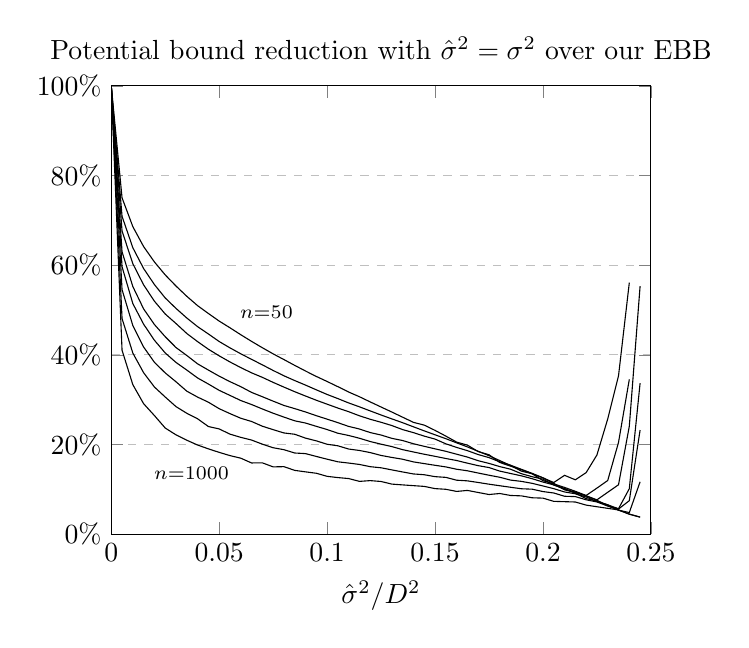
\begin{tikzpicture}
	\begin{axis}[
		title={Potential bound reduction with $\hat{\sigma}^2 = \sigma^2$ over our EBB},
		xlabel={$\hat{\sigma}^2/D^2$},
		xmin=0, xmax=0.25,
		ymin=0, ymax=100,
		xtick={0,0.05,0.1,0.15,0.2,0.25},
		ytick={0,20,40,60,80,100},
		yticklabel=$\pgfmathprintnumber{\tick}\%$,
		legend pos=south west,
		ymajorgrids=true,
		grid style=dashed,
		xticklabel style={/pgf/number format/fixed},
	]
	\addplot[] coordinates {
(0.0, 100.0)(0.005, 75.02420135527589)(0.01, 68.58202038924931)(0.015, 64.13237924865832)(0.02, 60.71118820468343)(0.025, 57.819103972950124)(0.03, 55.33498759305211)(0.035, 53.04630381803412)(0.04, 50.96)(0.045, 49.21383647798742)(0.05, 47.51937984496124)(0.055, 46.02446483180428)(0.06, 44.47806354009077)(0.065, 42.99625468164794)(0.07, 41.57386785449146)(0.075, 40.20618556701031)(0.08, 38.93352812271731)(0.085, 37.63596809282088)(0.09, 36.38328530259366)(0.095, 35.17191977077364)(0.1, 34.04558404558404)(0.105, 32.88447909284196)(0.11, 31.68666196189132)(0.115, 30.639494026704146)(0.12, 29.481792717086833)(0.125, 28.35195530726257)(0.13, 27.228412256267408)(0.135, 26.0778859527121)(0.14, 24.930555555555557)(0.145, 24.31129476584022)(0.15, 23.140495867768596)(0.155, 21.862068965517242)(0.16, 20.525224602626125)(0.165, 19.8489010989011)(0.17, 18.413793103448278)(0.175, 17.707618393960193)(0.18, 15.975103734439834)(0.185, 15.161957270847692)(0.19, 14.36426116838488)(0.195, 13.452299245024022)(0.2, 12.542837559972584)(0.205, 11.51473612063057)(0.21, 13.115845539280958)(0.215, 12.117177097203728)(0.22, 13.71280724450194)(0.225, 17.65424557116677)(0.23, 25.69558101472995)(0.235, 35.30794546309356)(0.24, 56.085994309200125)
		}node[pos=0.4](endofplotsquare){} ;
	\node [above right] at (endofplotsquare) {$\scriptstyle n=50$};
	\addplot[] coordinates {
(0.0, 100.0)(0.005, 70.89337175792507)(0.01, 63.881401617250674)(0.015, 59.23076923076923)(0.02, 55.66502463054187)(0.025, 52.67538644470868)(0.03, 50.345622119815665)(0.035, 48.20627802690583)(0.04, 46.2800875273523)(0.045, 44.646680942184155)(0.05, 42.96218487394958)(0.055, 41.54639175257732)(0.06, 40.22289766970618)(0.065, 38.983050847457626)(0.07, 37.75811209439528)(0.075, 36.50485436893204)(0.08, 35.31669865642994)(0.085, 34.25047438330171)(0.09, 33.23943661971831)(0.095, 32.18604651162791)(0.1, 31.152073732718893)(0.105, 30.228310502283104)(0.11, 29.257246376811594)(0.115, 28.39173405211141)(0.12, 27.475468331846567)(0.125, 26.572187776793623)(0.13, 25.704225352112676)(0.135, 24.84689413823272)(0.14, 23.93385552654482)(0.145, 23.03030303030303)(0.15, 22.155172413793103)(0.155, 21.28755364806867)(0.16, 20.35928143712575)(0.165, 19.453924914675767)(0.17, 18.46808510638298)(0.175, 17.502124044180118)(0.18, 16.397621070518266)(0.185, 15.306122448979592)(0.19, 14.054514480408859)(0.195, 13.463166807790008)(0.2, 11.925042589437819)(0.205, 11.205432937181664)(0.21, 10.414902624894157)(0.215, 9.551986475063398)(0.22, 8.622147083685546)(0.225, 10.262725779967159)(0.23, 11.961722488038278)(0.235, 20.45616535994298)(0.24, 34.51481696687972)
		}node[pos=0.693](endofplotsquare){} ;
	%\node [above] at (endofplotsquare) {$\scriptstyle n=75$};
	\addplot[] coordinates {
(0.0, 100.0)(0.005, 67.61904761904762)(0.01, 60.31468531468531)(0.015, 55.5921052631579)(0.02, 51.95618153364632)(0.025, 49.0990990990991)(0.03, 46.97406340057637)(0.035, 44.75524475524475)(0.04, 42.93478260869565)(0.045, 41.246684350132625)(0.05, 39.766839378238345)(0.055, 38.40304182509506)(0.06, 37.142857142857146)(0.065, 35.97560975609756)(0.07, 34.97005988023952)(0.075, 33.844339622641506)(0.08, 32.7906976744186)(0.085, 31.76605504587156)(0.09, 30.804077010192525)(0.095, 29.86577181208054)(0.1, 28.98230088495575)(0.105, 28.11816192560175)(0.11, 27.302275189599133)(0.115, 26.394849785407725)(0.12, 25.61105207226355)(0.125, 24.94736842105263)(0.13, 24.217118997912316)(0.135, 23.316062176165804)(0.14, 22.633744855967077)(0.145, 21.859039836567927)(0.15, 21.196754563894523)(0.155, 20.141700404858298)(0.16, 19.335347432024168)(0.165, 18.61861861861862)(0.17, 17.74675972083749)(0.175, 17.063492063492063)(0.18, 16.12265084075173)(0.185, 15.369458128078819)(0.19, 14.454277286135694)(0.195, 13.555992141453832)(0.2, 12.561334641805692)(0.205, 11.307767944936087)(0.21, 9.881422924901186)(0.215, 9.251968503937007)(0.22, 8.537782139352306)(0.225, 7.647058823529412)(0.23, 9.333333333333334)(0.235, 11.00832562442183)(0.24, 24.0625)(0.245, 55.32786885245902)
		}node[pos=1.0](endofplotsquare){} ;
	%\node [above] at (endofplotsquare) {$n=100$};
	\addplot[] coordinates {
(0.0, 100.0)(0.005, 62.98342541436464)(0.01, 55.223880597014926)(0.015, 50.23041474654378)(0.02, 46.753246753246756)(0.025, 44.03292181069959)(0.03, 41.61735700197239)(0.035, 39.84819734345351)(0.04, 37.981651376146786)(0.045, 36.58969804618117)(0.05, 35.233160621761655)(0.055, 34.00673400673401)(0.06, 32.89473684210526)(0.065, 31.612903225806452)(0.07, 30.647709320695103)(0.075, 29.658385093167702)(0.08, 28.702290076335878)(0.085, 27.994011976047904)(0.09, 27.245949926362297)(0.095, 26.41509433962264)(0.1, 25.644699140401148)(0.105, 24.858757062146893)(0.11, 24.022346368715084)(0.115, 23.448275862068964)(0.12, 22.646657571623464)(0.125, 22.10242587601078)(0.13, 21.36181575433912)(0.135, 20.871862615587848)(0.14, 20.157068062827225)(0.145, 19.58495460440986)(0.15, 19.02313624678663)(0.155, 18.471337579617835)(0.16, 17.825537294563844)(0.165, 17.189460476787954)(0.17, 16.375)(0.175, 15.77639751552795)(0.18, 15.061728395061728)(0.185, 14.478527607361963)(0.19, 13.480392156862745)(0.195, 12.804878048780488)(0.2, 12.257281553398059)(0.205, 10.94890510948905)(0.21, 10.194174757281553)(0.215, 9.101941747572816)(0.22, 7.907542579075426)(0.225, 7.38498789346247)(0.23, 6.521739130434782)(0.235, 5.669481302774427)(0.24, 10.136674259681094)(0.245, 33.693843594009984)
		}node[pos=1.0](endofplotsquare){} ;
	%\node [above] at (endofplotsquare) {$n=150$};
	\addplot[] coordinates {
(0.0, 100.0)(0.005, 59.642857142857146)(0.01, 51.41955835962145)(0.015, 46.820809248554916)(0.02, 43.24324324324324)(0.025, 40.40920716112532)(0.03, 38.292682926829265)(0.035, 36.5967365967366)(0.04, 34.831460674157306)(0.045, 33.47826086956522)(0.05, 32.06751054852321)(0.055, 30.942622950819672)(0.06, 29.8)(0.065, 28.90625)(0.07, 27.915869980879542)(0.075, 26.96629213483146)(0.08, 26.102941176470587)(0.085, 25.270758122743683)(0.09, 24.778761061946902)(0.095, 24.041811846689896)(0.1, 23.32761578044597)(0.105, 22.504230118443317)(0.11, 22.0)(0.115, 21.38157894736842)(0.12, 20.650406504065042)(0.125, 20.064205457463885)(0.13, 19.523809523809526)(0.135, 18.838304552590266)(0.14, 18.322981366459626)(0.145, 17.81874039938556)(0.15, 17.35159817351598)(0.155, 16.867469879518072)(0.16, 16.417910447761194)(0.165, 15.828402366863905)(0.17, 15.27165932452276)(0.175, 14.847161572052402)(0.18, 14.057971014492754)(0.185, 13.525179856115107)(0.19, 13.0)(0.195, 12.357954545454545)(0.2, 11.614730878186968)(0.205, 10.985915492957746)(0.21, 10.0)(0.215, 9.396914446002805)(0.22, 8.531468531468532)(0.225, 7.5524475524475525)(0.23, 6.3113604488078545)(0.235, 5.594405594405594)(0.24, 7.462686567164179)(0.245, 23.214285714285715)
		}node[pos=1.0](endofplotsquare){} ;
	%\node [above] at (endofplotsquare) {$n=200$};
	\addplot[] coordinates {
(0.0, 100.0)(0.005, 54.54545454545455)(0.01, 46.52173913043478)(0.015, 41.732283464566926)(0.02, 38.32116788321168)(0.025, 35.95890410958904)(0.03, 33.980582524271846)(0.035, 31.888544891640866)(0.04, 30.56379821958457)(0.045, 29.428571428571427)(0.05, 27.977839335180054)(0.055, 26.881720430107528)(0.06, 25.848563968668408)(0.065, 25.126903553299492)(0.07, 24.069478908188586)(0.075, 23.300970873786408)(0.08, 22.565320665083135)(0.085, 22.273781902552205)(0.09, 21.4123006833713)(0.095, 20.80536912751678)(0.1, 20.044052863436125)(0.105, 19.696969696969695)(0.11, 18.976545842217483)(0.115, 18.658280922431867)(0.12, 18.181818181818183)(0.125, 17.551020408163264)(0.13, 17.10261569416499)(0.135, 16.69980119284294)(0.14, 16.110019646365423)(0.145, 15.728155339805825)(0.15, 15.355086372360844)(0.155, 14.990512333965844)(0.16, 14.473684210526315)(0.165, 14.12639405204461)(0.17, 13.627992633517495)(0.175, 13.138686131386862)(0.18, 12.681159420289855)(0.185, 12.050359712230216)(0.19, 11.764705882352942)(0.195, 11.327433628318584)(0.2, 10.73943661971831)(0.205, 10.13986013986014)(0.21, 9.40766550522648)(0.215, 8.996539792387543)(0.22, 8.290155440414507)(0.225, 7.253886010362694)(0.23, 6.540447504302926)(0.235, 5.344827586206897)(0.24, 4.810996563573883)(0.245, 11.67192429022082)
		}node[pos=1.0](endofplotsquare){} ;
	%\node [above] at (endofplotsquare) {$n=300$};
	\addplot[] coordinates {
(0.0, 100.0)(0.005, 48.091603053435115)(0.01, 40.38461538461539)(0.015, 36.0)(0.02, 32.8125)(0.025, 30.58252427184466)(0.03, 28.440366972477065)(0.035, 26.956521739130434)(0.04, 25.726141078838175)(0.045, 24.0)(0.05, 23.46153846153846)(0.055, 22.304832713754646)(0.06, 21.58273381294964)(0.065, 20.97902097902098)(0.07, 20.068027210884352)(0.075, 19.269102990033222)(0.08, 18.83116883116883)(0.085, 18.095238095238095)(0.09, 17.956656346749227)(0.095, 17.325227963525837)(0.1, 16.71641791044776)(0.105, 16.129032258064516)(0.11, 15.85014409221902)(0.115, 15.536723163841808)(0.12, 15.041782729805014)(0.125, 14.794520547945206)(0.13, 14.324324324324325)(0.135, 13.866666666666667)(0.14, 13.421052631578947)(0.145, 13.246753246753247)(0.15, 12.820512820512821)(0.155, 12.658227848101266)(0.16, 12.030075187969924)(0.165, 11.881188118811881)(0.17, 11.519607843137255)(0.175, 11.138014527845037)(0.18, 10.79136690647482)(0.185, 10.451306413301662)(0.19, 10.117647058823529)(0.195, 10.023310023310023)(0.2, 9.49074074074074)(0.205, 9.174311926605505)(0.21, 8.447488584474886)(0.215, 8.371040723981901)(0.22, 7.657657657657658)(0.225, 7.174887892376682)(0.23, 6.263982102908278)(0.235, 5.369127516778524)(0.24, 4.464285714285714)(0.245, 3.7861915367483294)
		}node[pos=1.0](endofplotsquare){} ;
	%\node [above] at (endofplotsquare) {$n=500$};
	\addplot[] coordinates {
(0.0, 100.0)(0.005, 41.02564102564103)(0.01, 33.333333333333336)(0.015, 29.09090909090909)(0.02, 26.446280991735538)(0.025, 23.66412213740458)(0.03, 22.142857142857142)(0.035, 20.945945945945947)(0.04, 19.871794871794872)(0.045, 19.01840490797546)(0.05, 18.235294117647058)(0.055, 17.51412429378531)(0.06, 16.939890710382514)(0.065, 15.873015873015873)(0.07, 15.897435897435898)(0.075, 15.0)(0.08, 15.048543689320388)(0.085, 14.218009478672986)(0.09, 13.88888888888889)(0.095, 13.574660633484163)(0.1, 12.88888888888889)(0.105, 12.608695652173912)(0.11, 12.393162393162394)(0.115, 11.764705882352942)(0.12, 11.934156378600823)(0.125, 11.740890688259109)(0.13, 11.155378486055778)(0.135, 10.980392156862745)(0.14, 10.81081081081081)(0.145, 10.64638783269962)(0.15, 10.150375939849624)(0.155, 10.0)(0.16, 9.523809523809524)(0.165, 9.747292418772563)(0.17, 9.285714285714286)(0.175, 8.8339222614841)(0.18, 9.059233449477352)(0.185, 8.620689655172415)(0.19, 8.532423208191126)(0.195, 8.108108108108109)(0.2, 8.02675585284281)(0.205, 7.308970099667774)(0.21, 7.2368421052631575)(0.215, 7.166123778501628)(0.22, 6.472491909385114)(0.225, 6.109324758842444)(0.23, 5.7507987220447285)(0.235, 5.396825396825397)(0.24, 4.444444444444445)(0.245, 3.7974683544303796)
		}node[pos=0.85](endofplotsquare){} ;
	\node [below left] at (endofplotsquare) {$\scriptstyle n=1000$};
	\end{axis}
	\end{tikzpicture}
	\vspace{-10pt}
	\caption{The percent reduction in the 0.5 probability bound}
	\label{biggraph4}
\end{figure}
\end{frame}


\section{Possible Improvements}

\begin{frame}
\frametitle{Possible Improvements?}
\begin{itemize}
\item Can we avoid Union Bounds? need to develop bounds on coincidence of variance bounds being violated and sample-mean bound being violated.
\item Can we develop stronger Entropic bounds specifically for the variance function?
\item Can we develop use numerical methods to -directly- solve the question, qua. Optimal Uncertainty Quantification.
\item Can we create bounds that take advantage of sampling \textit{without} replacement? not assuming the i.i.d of samples.
\item Can we extend to multidimensional data?
\item Can we extend to different (non-simple-random) sampling schemes? eg. snowball, stratified, cluster sampling.
\end{itemize}
The first three, I dont know. the second three, definitely yes.
\end{frame}


\begin{frame}
\begin{Theorem}[Vector SEBM bound]
%In the context above, then with $\Omega_{m_i}^{n_i},\Psi_{m_i}^{n_i}$ per Lemma~\ref{martingale1}:
\begin{equation*}\label{big_equation2}\pr\left(\begin{matrix*}[l]\sum_{j=1}^M\left(\sum_{i=1}^n\tau_i(\chi_{i,m_i,j}-\mu_{i,j})\right)^2 \ge \\ \quad\quad \log(6/p)\sum_{j=1}^M\left(\alpha_{m_i,j}^{n_i} +\left(\sqrt{\beta_{m_i,j}^{n_i}} +\sqrt{\gamma_{m_i,j}^{n_i}}\right)^2\right)\end{matrix*} \right)\le Mp \end{equation*}
where:\\
$\alpha_{j}=\sum_{i=1}^n\frac{4}{17}\Omega_{m_i}^{n_i}D_{i,j}^2\tau_i^2 $ \\
$\beta_{j}=\log(3/p)\left(\max_i\tau_i^2{\Psi_{m_i}^{n_i}}^2D_{i,j}^2\right) $ \\
$\gamma_{j}=2\sum_{i=1}^n\tau_i^2\Psi_{m_i}^{n_i}(m_i-1)\doublehat{\sigma}_{i,j}^2/m_i$
$+ \log(6n/p)\sum_i\tau_i^2D_{i,j}^2\Omega_{m_i}^{n_i}\Psi_{m_i}^{n_i} $ \\
$\quad\quad\quad\quad\quad\quad\quad\quad\quad\quad\quad\quad\quad\quad~~+\log(3/p)\left(\max_i\tau_i^2{\Psi_{m_i}^{n_i}}^2D_{i,j}^2\right)$\\
where:\\
$\bar{\Omega}_m^n = \sum_{k=m}^{n-1}\frac{1}{k^2}\approx \frac{(m+1)(1-m/n)}{m^2}$\\
$\bar{\Psi}_m^n = \sum_{k=m}^{n-1}\frac{n}{k^2(k+1)}\approx \frac{n+1-m}{m^2}$
\end{Theorem}
\end{frame}

\begin{frame}
For more info:\\
``Stratied Finite Empirical Bernstein Sampling''
https://www.preprints.org/manuscript/201901.0202/v2\\
\-\hspace{1cm}\\
Questions?
\end{frame}


%------------------------------------------------

\begin{frame}
%\frametitle{References}
%\bibliographystyle{plain}
\bibliographystyle{authordate1}
\bibliography{bib}


%\footnotesize{
%\begin{thebibliography}{99} % Beamer does not support BibTeX so references must be inserted manually as below
%\bibitem[Smith, 2012]{p1} John Smith (2012)
%\newblock Title of the publication
%\newblock \emph{Journal Name} 12(3), 45 -- 678.
%\end{thebibliography}
%}
\end{frame}







\end{document} 
